\newpage
\section{THEORETICAL PART}

%%%%%%%%%%%%%%%%%%%%%%%%%%%%%%%%%%%%%%%%%%%%%%%%%%%%%%%%%%%%%%%%%%%%%%%%%%%%%%%%%%%%%%%%
%%%%%%%%%%%%%%%%%%%%%%%%%%%%%%%%%%%%%%%%%%%%%%%%%%%%%%%%%%%%%%%%%%%%%%%%%%%%%%%%%%%%%%%%
\subsection{Molecular dynamics}
The molecular dynamics method is based on solving the equations of motion of classical Newtonian mechanics for atoms. Let us choose the assumption that the interaction potential $U$ is continuous and differentiable. The force acting on the $i$ particle can thus be written as an equation \ref{sila1} 
\begin{equation}\label{sila1}
	f_i=-\frac{\partial U(r^N)}{\partial r_i}, \qquad i=1,...,N.
\end{equation}

In molecular dynamics, we are focused on the time development of the model. In the other words, we are looking for the trajectory of the solution of the respective systems of differential equations. In Newtonian mechanics, acceleration is directly related to forces through the equations of motion. Formally, we can write the equation \ref{sila2}
\begin{equation}\label{sila2}
	\Ddot{r_i}=\frac{f_i}{m_i}, \qquad i=1,...,N,
\end{equation}
where the second time derivative of the positions appears on the left side. The equation \ref{sila2} is a system of 3$N$ ordinary differential equations for a set of $N$ atoms. As initial conditions, we usually choose knowledge of all positions $r_i$ and velocities $\dot{r_i}$ at the initial time $t=t_0$. 

We solve equation \ref{sila2} using the finite difference method when we track the desired solution in the form of the function $r_i(t), i=1,..,N$, in the time interval $[t_0,t_{max}]$ at discrete points of the form $t=t_0+kh$, where $h$ is the integration step and $k$ is a non-negative integer.

To find a solution, it is necessary to calculate the forces acting on individual particles at each step of the simulation. One of the methods that is applied in this area is the Verlet integration method. It is a simple and very effective method that provides sufficiently accurate results. Its great advantage is the reversibility of time and the conservation of the total energy of the system~\cite{mdskripta}.

\subsubsection{Verlet integration}
Verlet integration method is a numerical method for integrating the equation \ref{sila1}. We express the second derivative using finite differences. From the second-order Taylor expansion $r_i(t\pm h)$ centred at $t$, we obtain the formula
\begin{equation}\label{sila3}
	\Ddot{r_i}=\frac{r_i(t-h)-2r_i(t)+r_i(t+h)}{h^2},
\end{equation}
binding values at three points in a row ($t-h$, $t$ and $t+h$). We will use this characteristic to calculate $r_i(t+h)$. By substituting \ref{sila3} into \ref{sila1} we get 
\begin{equation}\label{sila4}
	r_i(t+h)=2r_i(t)-r_i(t-h)+h^2\frac{f_i(t)}{m_i}.
\end{equation}
In this formulation, we are able to calculate the new positions at time $t+h$ from knowledge of the forces at time $t$, the positions of the particles at time $t$ and the previous time $t-h$. The time reversibility of the method is clearly visible here. The advantage is that the force is calculated only once in each step of the simulation. For the position preceding the initial position ($r_i(t_0-h)$), we can use the expansion \ref{sila5}
\begin{equation}\label{sila5}
	r_i(t_0-h)=r_i(t)-h\dot{r_i}(t_0)+h^2\frac{f_i(t_0)}{2m_i}.
\end{equation}

\subsubsection{Velocity Verlet}

\subsubsection{Constraint dynamics}

When integrating equations of motion, we often impose the condition of conservation of variables. The main reason is the optimal choice of the simulation time step. If we simulate with too large time step, we introduce large errors into the simulations, leading in extreme cases to a crash of the simulation. The calculated particle positions at time $t+h$ may lead to overlapping of particles, the calculated force acting on the particles may then bring the particles back to the overlapping region or eject the particles far from their natural position. Conversely, the use of inappropriately short simulation steps reduces the efficiency of the simulations (the most computationally and therefore time consuming element of the simulations is the calculation of the forces when integrating the equations of motion). The criterion determining the optimal step length is the accuracy of the conservation of total energy. The step length can be determined by an Nyquist sampling theorem that says that the time step must be half or less of the period of the quickest dynamics. Thus, for systems containing very light hydrogen atoms, we can either artificially increase the mass of the hydrogen atom while redistributing the masses of the other molecules to conserve the overall mass of the molecule, or fix the bond angles or bond lengths terminating in the hydrogen atoms. It is the fixation of hydrogen bond lengths that is most often implemented in the Verlet method, using an algorithm called SHAKE. Fixing the bond length allows us to use a longer time step (we are no longer limited by the motion of very light particles) and, unlike fixing angles, does not introduce large deviations in the simulations.

\subsubsection{SHAKE algorithm}

The SHAKE algorithm is based on Verlet's integration method and is iterative. The first step is to initialize the initial velocities and positions of the atoms, then calculate the positions using Verlet's method without considering bond length constraint. We then create the $\lambda$ correction of the atom positions to constrain the bond length, which we calculate by considering the correct bond length between atoms i and j from the condition 

\begin{equation}\label{SHAKE}
	[\vec{r}_{\text{Verlet},ij}(t + h)-\lambda\vec{r}_{ij}(t)]^2 = \vec{r}_{ij}(t)^2,
\end{equation}
where Verlet index comes from previously described Equation \ref{sila4} for Verlet method. When we consider After omitting the we can calculate $\lambda$ as

\begin{equation}\label{SHAKE_lamda}
	\lambda \approx \frac{|\vec{r}_{\text{Verlet},ij}(t + h)|^2 - |\vec{r}_{ij}(t)|^2}
	{2\vec{r}_{\text{Verlet},ij}(t + h) \cdot \vec{r}_{ij}(t)}
\end{equation}

\begin{equation}\label{SHAKE_lamdai}
	\vec{r}_i(t + h) = \vec{r}_{\text{Verlet},i}(t + h) + \lambda \frac{1/m_i}{ 1/m_i + 1/m_j} \vec{r}_{ij}
\end{equation}

\begin{equation}\label{SHAKE_lamdaj}
	\vec{r}_j(t + h) = \vec{r}_{\text{Verlet},j}(t + h) - \lambda \frac{1/m_j}{ 1/m_i + 1/m_j} \vec{r}_{ij}
\end{equation}

\subsection{title}
\subsection{Silová pole}

In order to convert a real system consisting of individual molecules into a form that can be understood by computer software, we must define the individual parameters that are essential for calculating interactions. The set of parameters thus calculated is called the force field. Let us discuss the individual members that make up this field. First we approximate the individual atoms by spheres, each such sphere will be represented by its mass. We then have to figure out how to represent the bonds and interatomic interactions. Classical force fields contain the sum of the individual contributions broken down in terms described by Equation \ref{ff}.

To get a better idea of what lies behind the individual terms, let us present a modified figure taken from:  In the following paragraphs, the individual terms will be described in more detail.

\begin{figure}[htb!]
	\centering
	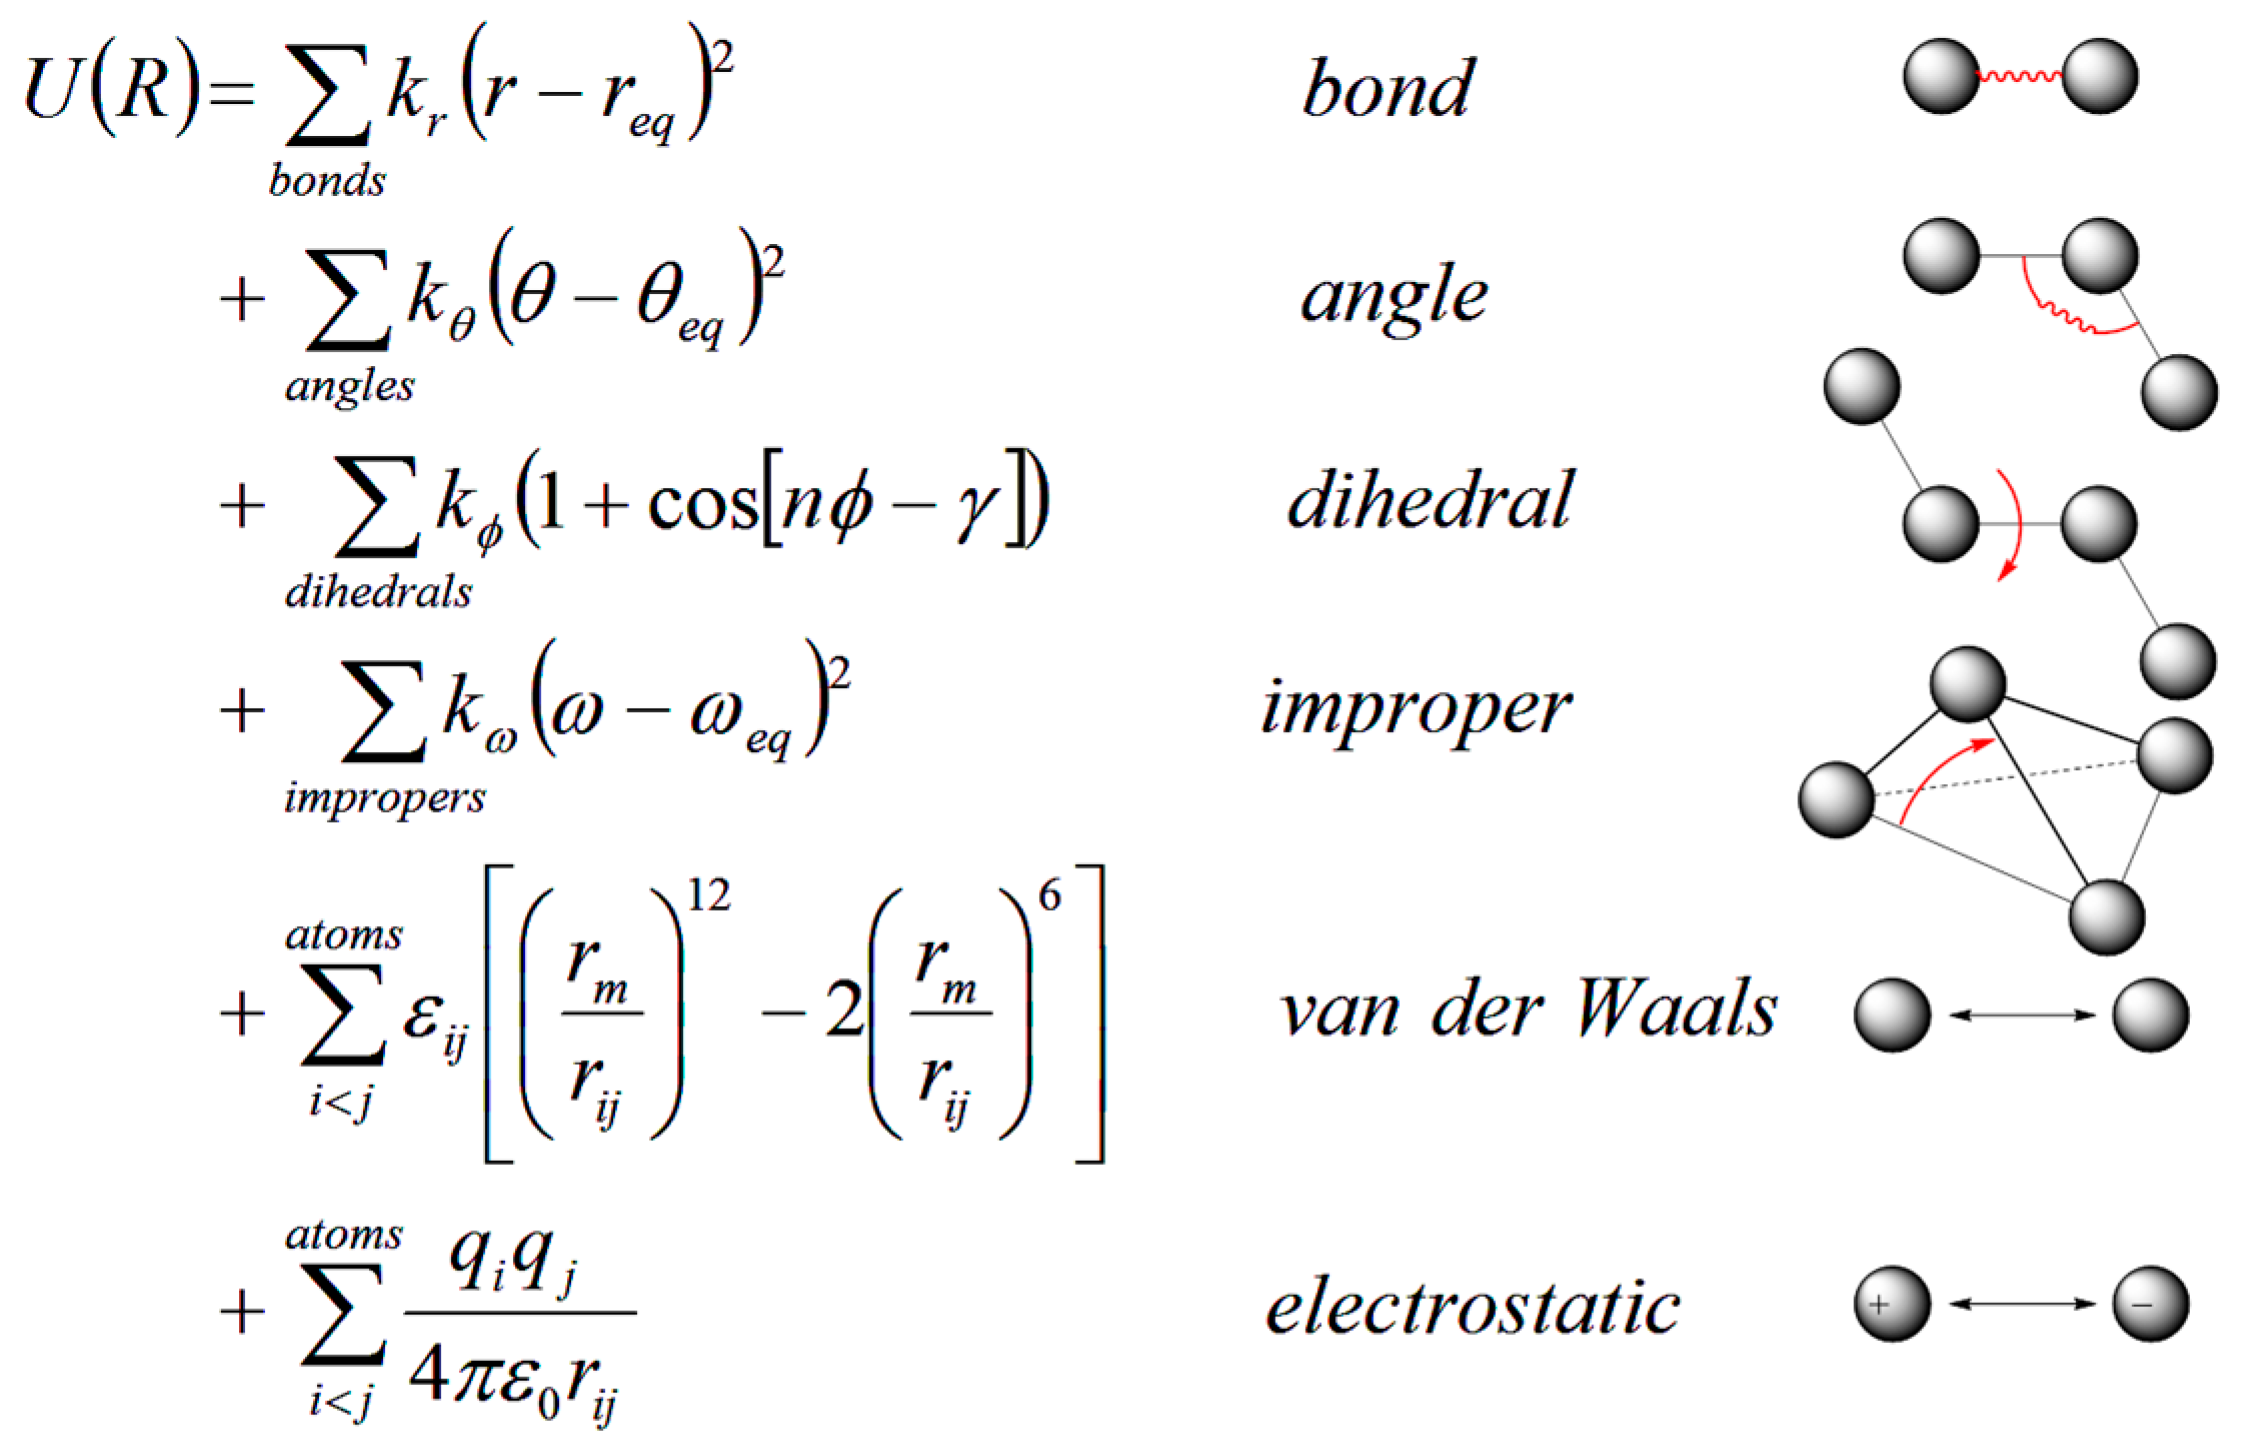
\includegraphics[width=1.0\linewidth]{img/ff.png} 
	\caption{caption}
	\label{fig:ff}    
\end{figure}  




\subsection{Polarizovaná silová pole}